\clearpage
\Question{A New Implementation of Queues}

Recall the interface for a stack that stores
elements of the type \lstinline'elem':

\begin{quote}
\begin{lstlisting}
// typedef ______* stack_t;

bool stack_empty(stack_t S)              /* O(1) */
/*@requires S != NULL; @*/;

stack_t stack_new()                      /* O(1) */
/*@ensures \result != NULL; @*/
/*@ensures stack_empty(\result); @*/;

void push(stack_t S, elem x)             /* O(1) */
/*@requires S != NULL; @*/;

elem pop(stack_t S)                      /* O(1) */
/*@requires S != NULL; @*/
/*@requires !stack_empty(S); @*/;
\end{lstlisting}
\end{quote}

For this question you will analyze a different implementation of the
queue interface. Instead of a linked list, this implementation uses
two stacks, called \lstinline'instack' and \lstinline'outstack'. To
enqueue an element, we push it on top of the \lstinline'instack'. To
dequeue an element, we pop the top off of the \lstinline'outstack'. If
the \lstinline'outstack' is empty when we try to dequeue, then we will
first move all of the elements from the \lstinline'instack' to
the \lstinline'outstack', then pop the \lstinline'outstack'.

For example, below is one possible configuration of a two-stack queue
containing the elements \lstinline'A' through \lstinline'E' (\lstinline'A' is
at the front and \lstinline'E' is at the back of the abstract queue):
\begin{center}
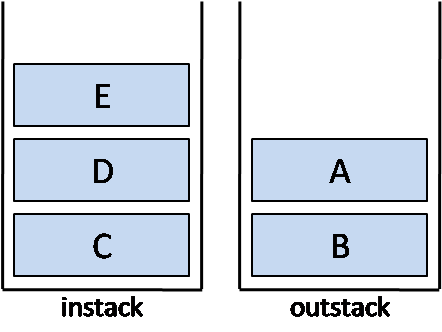
\includegraphics[width=0.3\linewidth]{\img/twostack-queue.png}
\end{center}

We will use the following C0 code:

\begin{lstlisting}[numbers=none]
typedef struct stackqueue_header stackqueue;
struct stackqueue_header {
  stack_t instack;
  stack_t outstack;
};

typedef stackqueue* queue_t;
\end{lstlisting}
\clearpage
\begin{lstlisting}[numbers=none]
bool is_stackqueue(stackqueue* Q) {
  return Q != NULL && Q->instack != NULL && Q->outstack != NULL;
}

stackqueue* queue_new()
//@ensures is_stackqueue(\result);
{
  stackqueue* Q = alloc(stackqueue);
  Q->instack = stack_new();
  Q->outstack = stack_new();
  return Q;
}

bool queue_empty(stackqueue* Q)
//@requires is_stackqueue(Q);
//@ensures is_stackqueue(Q);
{
  return stack_empty(Q->instack) && stack_empty(Q->outstack);
}

void enq(stackqueue* Q, elem x)
//@requires is_stackqueue(Q);
//@ensures is_stackqueue(Q);
{
   push(Q->instack, x);
}

elem deq(stackqueue* Q)
//@requires is_stackqueue(Q);
//@requires !queue_empty(Q);
//@ensures is_stackqueue(Q);
{
    if (stack_empty(Q->outstack)) {
       while (!stack_empty(Q->instack))
         push(Q->outstack, pop(Q->instack));
    }
    return pop(Q->outstack);
}
\end{lstlisting}

\begin{parts}

\part[0\half]\TAGS{queue, stack}
Given a queue with $k$ elements in it, exactly how many different ways
can this queue be represented using two stacks, as a function of $k$?

\begin{framed}
\bigskip
\uanswer{12em}{$k+1$} way(s).
\end{framed}

\RUBRIC
Part (a)
TAGS: queue, stack

Gradescope rubric:
+ 0.5 pt k+1

Commentary:
k+1, all or nothing

ENDRUBRIC


\bigskip
\part[1]\TAGS{complexity, queue, stack}
We now determine the runtime complexity of the \lstinline'enq' and
\lstinline'deq' operations. Let $k$ be the total number of elements in
the queue.

What is the worst-case runtime complexity of each of the following
queue operations based on the description of the data structure
implementation given above? Write ONE sentence that explains each
answer.

\begin{framed}
\medskip
\lstinline'enq': \  $O(\uanswer{6em}{$1$})$, \ because
\uanswer{19.8em}{we always do exactly one push.\hfill}

\smallskip
\uanswer{34em}{}

\bigskip
\lstinline'deq': \  $O(\uanswer{6em}{$k$})$, \ because
\uanswer{19.8em}{we may need to pop all $k$ elements from\hfill}

\smallskip
\uanswer{34em}{the \lstinline'instack'.\hfill}
\end{framed}

\RUBRIC
Part (c)
TAGS: complexity, queue, stack

Gradescope rubric:
+ 0.5 pts enq is O(1) and some reasonable explanation
+ 0.5 pts deq is O(k) and some reasonable explanation

Commentary:
  +1/2pt: enq is O(1) and some reasonable explanation
  +1/2pt: deq is O(k) and some reasonable explanation
          Note that O(n) is NOT okay, function is in terms of k
ENDRUBRIC

\enlargethispage{3ex}
\part[2\half]\TAGS{amortized-cost}
Using amortized analysis, we can show that the worst-case complexity
of a \emph{valid sequence} of $n$ enqueue/dequeue operations starting
from an empty queue is $O(n)$.  This means that the amortized cost per
operation is $O(1)$, even though the worst-case cost of an individual
operation may not be constant.

Here, a \emph{valid sequence} of queue operations must start with the
empty queue, each operation must be either an \lstinline'enq' or a
\lstinline'deq', and you must have enough tokens.  Assume that
\lstinline'push' and \lstinline'pop' each consume one token (and
emptiness tests are free).

How many tokens should be charged to enqueue an element? How many to
dequeue an element?  Your answers should be constant integers ---
recall that the amortized cost is to be $O(1)$.  Justify each answer
by briefly stating for what purpose of each token is used (\emph{you
  may not need all lines}).

\begin{framed}
\newcommand{\tokenPurpose}[1]{\item[1] token to \uanswer{27.5em}{#1\hfill}}
\medskip
Cost of \lstinline{enq}: \uanswer{8em}{3} token(s), to be used as follows:
\begin{itemize}
\tokenPurpose{push instack}
\tokenPurpose{pop instack}
\tokenPurpose{push outstack}
\tokenPurpose{}
%\tokenPurpose{}
\end{itemize}

\bigskip
Cost of \lstinline{deq}: \uanswer{8em}{1} token(s), to be used as follows:
\begin{itemize}
\tokenPurpose{pop outstack}
\tokenPurpose{}
\tokenPurpose{}
\tokenPurpose{}
%\tokenPurpose{}
\end{itemize}
\end{framed}


\RUBRIC
Part (d)
TAGS: amortized-cost

Gradescope rubric:
+1.5pt First box number and explanation correct: EITHER 3: push-instack, pop-instack, push-outstack OR 4: push-instack, pop-instack, push-outstack, pop-outstack
+1pt Second box number and explanation correct: depending on answer to first box, EITHER 1: pop-outstack OR 0

Commentary:
Doesn't have to match their implementation.
  +1.5pt - Correct token numbers (3/1 or 4/0). No partial credit.
  +1pt - Correct assignment of tokens to operations. No partial credit
  unless you see a compelling reason; consult with the staff if so.

  Expected answer:
    enqueue takes 3 (push-instack, pop-instack, push-outstack)
    dequeue takes 1 (pop-outstack)

  Alternate answer:
    enqueue takes 4 (push-instack, pop-instack, push-outstack, pop-outstack)
    dequeue takes 0
ENDRUBRIC

\end{parts}
